\documentclass[12pt]{article}
\usepackage[left=2cm, top=1cm, right=2cm, bottom=2cm]{geometry}
\usepackage[utf8]{inputenc}      % accents dans le source
\usepackage[T1]{fontenc}
\usepackage[french]{babel}
\usepackage{graphicx}
\usepackage{graphics}
\usepackage{amsmath}
\usepackage{tikz}
\usepackage{xcolor} 
\usepackage{mathtools}
\usepackage{parskip}
\usepackage{subcaption}
\usepackage[export]{adjustbox}

\title{\textbf{TP 1 - Electrostatique}}
\author{MENARD Alexandre - VIEILLEDENT Florent}
\setlength{\parindent}{1cm}
\date{}
\begin{document}
\maketitle

L'électrostatique est le domaine de l'électromagnétisme qui étudie les champs électrique permanent, qui ne dépendent pas du temps. L'électrostatique induit de nombreux phénomènes physiques,
le plus intéressant étant de comprendre les liens entre ces derniers. Par exemple, l'électroscope et le filet d'eau attiré par un ballon chargé en le frottant contre un tissu partagent la même origine: les forces de Coulomb où un amas de charges vont attirer les molécules d'eau formant un dipôle.
Dans ce travail pratique, on cherchera à vérifier l'équation de Laplace et la formule pour la capacité d'un condensateur plan. 
Pour la première loi, on mesurera le potentiel entre des électrodes circulaires et pour la deuxième on étudiera la décharge du condensateur avec un oscilloscope.

\section{Potentiel électrostatique généré par des électrodes circulaire}
	\subsection{Modèle}
	\label{section:laplacien}
	On se place dans le cadre d'un régime permanent où les électrodes sont à l'équilibre. Les charges se retrouvent donc à la surface des électrodes, d'où $\rho(M) = 0$, et ceux pour tout point $M$.
	L'équation de Laplace nous donne $\Delta V(M) = 0$, avec $\Delta V(M)$ l'opérateur Laplacien. 
	Les électrodes étant circulaires, la répartition des charges est invariant par rotation autour de $Oz$ et on néglige la variation de $V(M)$ selon $z$, donc $V(r,\theta, z)=V(r)$\footnote{La répartition des charges provoque la présence d'une d.d.p, on retrouve effectivement le principe de Curie où la cause et l'effet présentent la même symétrie par rotation autour de $Oz$}, on s'attend à des équipotentielles circulaire.
	On privilégiera un référentiel polaire centré sur l'électrode centrale de part les symétries du problème
	
	Sous l'ensemble de ses hypothèses, la résolution (voir \ref{section:demonstration_laplacien}) de l'équation différentielles aux dérivées partielles nous donne alors le potentiel :
	\begin{align*}
		V(r) = \frac{V(R_2) - V(R_1)}{\ln(\frac{R_2}{R_1})} \ln\left(\frac{r}{R_1}\right) + V(R_1), V(r) \text{ croissant vers les rayons croissants}
	\end{align*}

	Pour le modèle, nous négligeons les variations de potentiel sur $z$, cependant les électrodes ne sont pas très hautes devant leurs rayons. Pour respecter cette limite, nous nous efforcerons de réaliser
	les mesures sur une même hauteur (en mesurant sur le papier carboné). Nous vérifierons expérimentalement si cette hypothèse est raisonnable.
	
	\subsection{Protocole expérimental}
	On fixe deux électrodes circulaire en aluminium sur du plastique isolant. L'électrode circulaire a un diamètre intérieur $d_{int} = 160,0 \pm 1 mm$ et un diamètre extérieur $d_{ext} = 180,0\pm 1 mm$.
	L'électrode intérieure est pleine de diamètre $d=15,0\pm 1 mm$. L'incertitude de la règle étant de $0.5mm$, l'incertitude du diamètre se voit doublée.
	
	Sur une plaque de plastique isolant, on dispose un papier carbonée (de conductivité faible devant les électrodes). On place ensuite les électrodes de manière concentrique 
	où celle la plus extérieure est reliée à la borne positive d'une alimentation continue de tension $U_0 = 15.008 \pm 0.005V$ (incertitude déterminée par la moyenne entre le potentiel maximal et minimal mesuré, et l'on utilisera cette même méthode pour les prochaines mesures), et celle interne reliée à la masse.
	On relèvera les potentiels en reliant le voltmètre à l'électrode centrale et à une sonde au point considéré, et la distance à l'aide d'une webcam. On tracera d'abord deux courbes d'équipotentielles $V_1 = 11V$ et $V_2 = 13V$, puis on relèvera environ $15$ potentiels
	à des rayons différents en augmentant le nombre de mesures lorsqu'on s'approche de l'électrode centrale pour suivre au plus proche le comportement du potentiel en $\ln(r)$. On attribuera une incertitude de $0.1cm$ pour le rayon de part la faible qualité de la caméra.
	
	\subsection{Résultats et interprétation}
	\begin{figure}[!htbp]
		\centering
		\subfloat[Courbe d'une équipotentielle]{\includegraphics[width=0.4\textwidth]{img/equi}\label{fig:f1}}
		\hfill
		\subfloat[Potentiel en fonction de $\ln(r/R_1)$.]{\includegraphics[width=0.6\textwidth]{img/ln_r.png}\label{fig:ln_r}}
		\caption{Résultat de l'expérience}
	\end{figure}
	Pour le tracé de l'équipotentielle, on remarque une légère différence de longueur d'axe entre l'axe entre les deux pinces crocodiles ($d_{croco-croco} \approx 3.8cm$), et l'axe perpendiculaire ($d_{\perp}\approx 4.25cm$).
	L'écart de rayon ne rentre pas en compte dans les incertitudes de mesures du rayon. Nous n'avons pas eu le temps de réaliser plusieurs fois la même expérience pour vérifier si l'erreur est systématique, mais cela pourrait venir de la variation de potentiel selon $z$. En effet, en relevant le potentiel à un rayon constant
	mais en appuyant ou non sur le papier (faisant donc très légèrement varier $z$ car le papier n'était pas parfaitement plat), on relève des écarts d'environ $0.1V$ pour les grands rayons à $0.3V$ pour les petits rayons.
	
	Pour l'évolution\footnote{Les incertitudes pour $V$ sont présentes mais trop petites pour être visible} de $V(r)$, on retrouve bien une droite affine quand on trace en fonction de $\ln(r/R_1)$, ce qui est en accord avec le modèle. Cependant,
	on remarque que le modèle n'est plus valide en $R_1$ où on observe des sauts de potentiels, d'où $V(R_1)$ qui ne rentre pas dans la régression linéaire\footnote{Nous n'avons pas affiché la régression linéaire prenant en compte le point en $R_1$ car la droite ne passait pas correctement dans les incertitudes, nous avons donc conclut que ce point extrémal était à exclure et demandait une explication de cette écart à la théorie.}.
	On obtient avec $V(R_1^+) = 2.43 \pm 0.01V$\footnote{$R_1$ ne faisant pas pas partie de la régression, on ne peut pas prendre en compte ce point pour les conditions limites ici} et $V(R_2) = 15.007 \pm 0.01V$:
	\begin{align*}
		\frac{V(R_2) - V(R_1^+)}{\ln(\frac{R_2}{R_1^+})} = 5.3 \pm 0.2 V \text{ et } a = \frac{V(R_2) - V(R_1^+)}{\ln(\frac{R_2}{R_1^+})} = 5.45 \pm 0.13 V
	\end{align*}

	On retrouve donc bien l'aspect qualitatif et quantitatif de la théorie en dehors de $r \leq R_1$.
	
\section{Mesure de capacité de condensateurs plans}
	\subsection{Modèle}
	La capacité $C$ d'un condensateur plan est donnée par $C = \frac{\epsilon_0 S}{h}$, $h$ la distance entre les deux plaques et $S$ la surface des plaques. Cette formule est valable pour des plaques infinies ce qui correspond à $h \ll S$.

	On applique la loi des mailles en notant $V$ la tension aux bornes du condensateur, lorsque le circuit est ouvert, on a:
	\begin{align*}
		V - V_{resistance} = 0 & \Rightarrow V - R_{oscilloscope}C \frac{dV}{dT} = 0 \Rightarrow V(t) = V_0 \exp(-t/\tau) + B
	\end{align*}

	Dans notre cas $V_0 = U_0$ la tension de l'alimentation et $R_{oscilloscope}$ la résistance de l'oscilloscope, et $B$ est le potentiel restant à la fin de la décharge.
	
	\subsection{Protocole expérimental}
	On dispose 4 pieds isolants où l'on positionne une plaque en aluminium de $350\times 350mm^2$. On dispose ensuite un jeu de 4 parallélépipèdes isolants de hauteur $h = 32, 10, 5, 3mm$ (après mesure, celui à $30mm$ fait en réalité $32mm$) puis
	on positionne une deuxième plaque identique à la première par dessus les parallélépipèdes isolants. On relie ensuite une plaque à la borne positive d'un générateur avec un interrupteur entre les deux, et on relie la seconde plaque à la masse.
	L'oscilloscope de résistance $R_{osc}=1 \pm 0.02 M\Omega$\footnote{L'incertitude est fournie dans le manuel} sera relié aux deux plaques pour mesurer la différence de potentiel entre les deux plaques.
	On appuie et maintient pendant 10 secondes le bouton pressoir pour charger le condensateur, et on relâche pour observer la décharge.
	
	\subsection{Résultats et interprétation}
	Pour les incertitudes, nous avons pris la moyenne de la différence entre deux mesures de potentiels successifs, et de même pour le temps à défaut d'informations dans le manuel de l'oscilloscope.
	On a donc $\delta U = 0.1V$ et $\delta t = 10^{-6}s$. Les courbes de décharges sont en annexe.
	Pour les quatres hauteurs, on obtient alors les résultats suivants après un fit de chacune des décharges:
	\begin{itemize}
		\item $h=32mm$, on a $U_0 = 15.011 \pm 0.1V, \tau = 8.99.10^{-5} \pm 10^{-9}s, B = 0.005 \pm 0.002V$
		\item $h=10mm$, on a $U_0 = 15.046 \pm 0.1V, \tau = 1.84.10^{-4} \pm 10^{-7}s, B = 0.005 \pm 0.004V$
		\item $h=5mm$, on a $U_0 = 15.00 \pm 0.1V, \tau = 2.58.10^{-4} \pm 10^{-7}s, B = 0.08 \pm 0.002V$
		\item $h=3mm$, on a $U_0 = 15.178 \pm 0.1V, \tau = 3.99.10^{-4} \pm 10^{-7}s, B = -0.07 \pm 0.001V$
	\end{itemize}
	\begin{figure}[!h]
		\centering
		\includegraphics[width=0.5\textwidth]{img/C_over_h.eps}
		\label{fig:Capacite}
		\caption{Capacité du condensateur selon l'inverse de la distance $h$}
	\end{figure}

	Nous obtenons alors:
	\begin{itemize}
		\item $C_{exp}(h) = \frac{a_1 }{h} + C_0$ avec $a_1 = (1.04 \pm 0.08).10^{-9} F.m^{-1}$ et $C_0 = (6.1 \pm 0.9) .10^{-11} F$
		\item $C_{th}(h) = \frac{a_2}{h} + C_{0_2}$ avec\footnote{L'incertitude sur $a_2$ n'est pas très cohérente car les points forment naturellement une droite de part sa définition dans notre cas} $a_2 = 1.08.10^{-9} \pm 4.10^{-18} F.m^{-1}$ et $C_{0_2} = (4.6 \pm 0.6) .10^{-18} F$
	\end{itemize}

	On note que les deux droites sont parallèles, cependant la capacité expérimentale est toujours plus haute que la capacité théorique d'une certaine valeur $C_0$ que l'on a déterminé. Cet écart est dû
	à une capacité parasite suite à la présence des fils et de l'oscilloscope, que l'on a déterminé et valant $C_0 = (6.1 \pm 0.9) .10^{-11} F$. Le fait que la capacité expérimentale est supérieure est d'ailleurs cohérent 
	car la capacité parasite ne peut qu'augmenter la capacité totale.

	Finalement, nous retrouvons bien le caractère qualitatif du modèle (un comportement linéaire selon $1/h$), mais la capacité totale du circuit prédite n'est pas en accord avec le modèle car ce dernier ne prend
	pas en compte les éléments composant le circuit autre que le condensateur. 
	
\section*{Conclusion}	
	Nous avons validé la forme des équipotentielles, ainsi que le comportement de $V(r)$ entre les deux électrodes malgré un écart à la théorie sur un point dont on arrive pas à proposer une explication satisfaisante. 
	On pourrait réaliser la même expérience avec une électrode interne plus petite et voir si les valeurs tendent plus vers le modèle en des rayons plus petits. De plus, les équipotentielles pourraient être plus précise en utilisant un papier
	présentant des cercles centrés sur l'électrode centrale et non gondolé. Concernant la capacité du condensateur, nous retrouvons bien le modèle à une capacité parasite près car le modèle ne prend en compte que le condensateur.

\break
\section*{Annexes}
	\subsection*{Constantes}
	Listes des constantes utilisées pour les calculs:
	\begin{itemize}
		\item $\epsilon_0 = 8,85.10^{-12} F.m^{-1}$
	\end{itemize}

	\subsection*{Démonstration de $\Delta V(M)$ dans \ref{section:laplacien}}
	\label{section:demonstration_laplacien}
	On se replace dans les hypothèses dans \ref{section:laplacien} à savoir:

	\begin{itemize}
		\item Régime permanent donc les charges sont à la surface des électrodes d'où $\rho (M) = 0$
		\item On néglige la variation du potentiel selon $z$
	\end{itemize}

	\begin{align*}
		\Delta V(M) = \frac{1}{r} \frac{\partial}{\partial r} \left( r \frac{\partial V(M)}{\partial r} \right) = 0 & \Rightarrow \frac{\partial V(M)}{\partial r} = \frac{C}{r} \\
		& \Rightarrow V(M) = C \ln(r) + V_0
	\end{align*}
	
	On a les conditions limites $V(R_1 = d)$ et $V(R_2 = d_{int})$ d'où:
	\begin{align*}
		V(R_1) = C \ln(R_1) + V_0 & \Rightarrow V_0 = V(R_1) - C \ln(R_1)
	\end{align*}
	\begin{align*}
		V(R_2) = C \ln(R_2) + V_0 & \Rightarrow C = \frac{V(R_2) - V_0}{\ln(R_2)} \\
		& \Rightarrow C = \frac{V(R_2) - V(R_1)}{\ln(R_2)} + C\frac{\ln(R_1)}{\ln(R_2)} \\
		& \Rightarrow C \left( 1 - \frac{\ln(R_1)}{\ln(R_2)}\right) = \frac{V(R_2) - V(R_1)}{\ln(R_2)} \\
		& \Rightarrow C = \frac{V(R_2) - V(R_1)}{\ln(\frac{R_2}{R_1})}
	\end{align*}

	Finalement, on trouve:
	\begin{align}
		\label{eqn:potentiel}
		V(r) = \frac{V(R_2) - V(R_1)}{\ln(\frac{R_2}{R_1})} \ln\left(\frac{r}{R_1}\right) + V(R_1)
	\end{align}
	
	\break
	
	\subsection*{Décharge des condensateurs}
	\begin{figure}[!h]
		\centering
		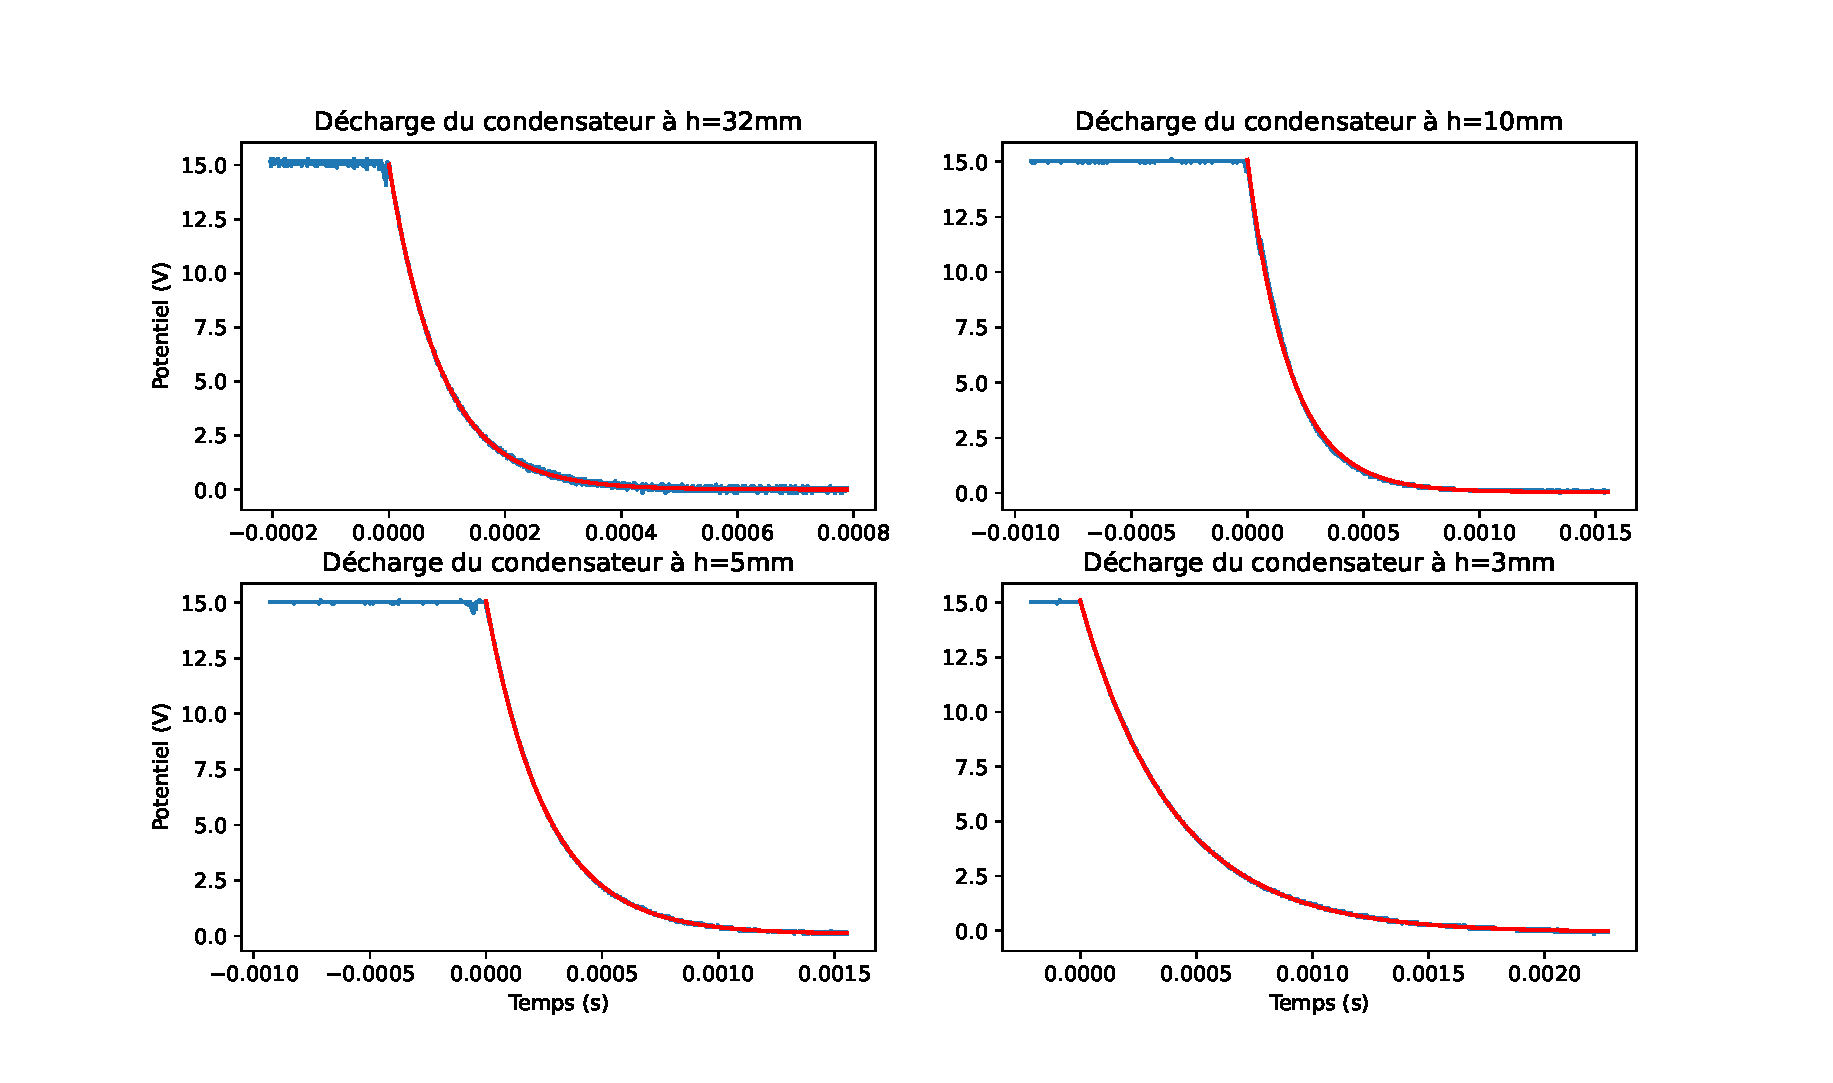
\includegraphics[width=1\textwidth]{img/decharge.eps}
		\label{fig:decharge}
		\caption{Décharge du condensateur au cours du temps selon la distance $h$}
	\end{figure}

\end{document}